\subsubsection{Software development methodologies used (D1)}
\label{methodology}

Software development methodology implies the process used for developing
particular software in a structured and methodical
way. We asked three questions: \begin{inparaenum}
\item Software development methodologies (Q6),
\item Requirements gathering (Q7), and
\item Most time-consuming software development activities (Q8).
\end{inparaenum}

\nd\bf{$\bullet$ Software development methodologies (Q6).} Agile is the most popular (64\%) development methodology in Bangladesh, followed by Scrum (46\%). These outcomes match the 2018 Stack Overflow
survey \citep{StackoverflowSurvey2018}, which also reports that Agile and Scrum
are the most popular methodologies worldwide. Among the other methodologies, 
pair programming (20\%) and Waterfall (12\%) are also popular in Bangladesh software companies.

\begin{figure}[t]
    \centering
    \caption{Software development methodologies used by the respondents}
    \begin{subfigure}{0.45\textwidth}
            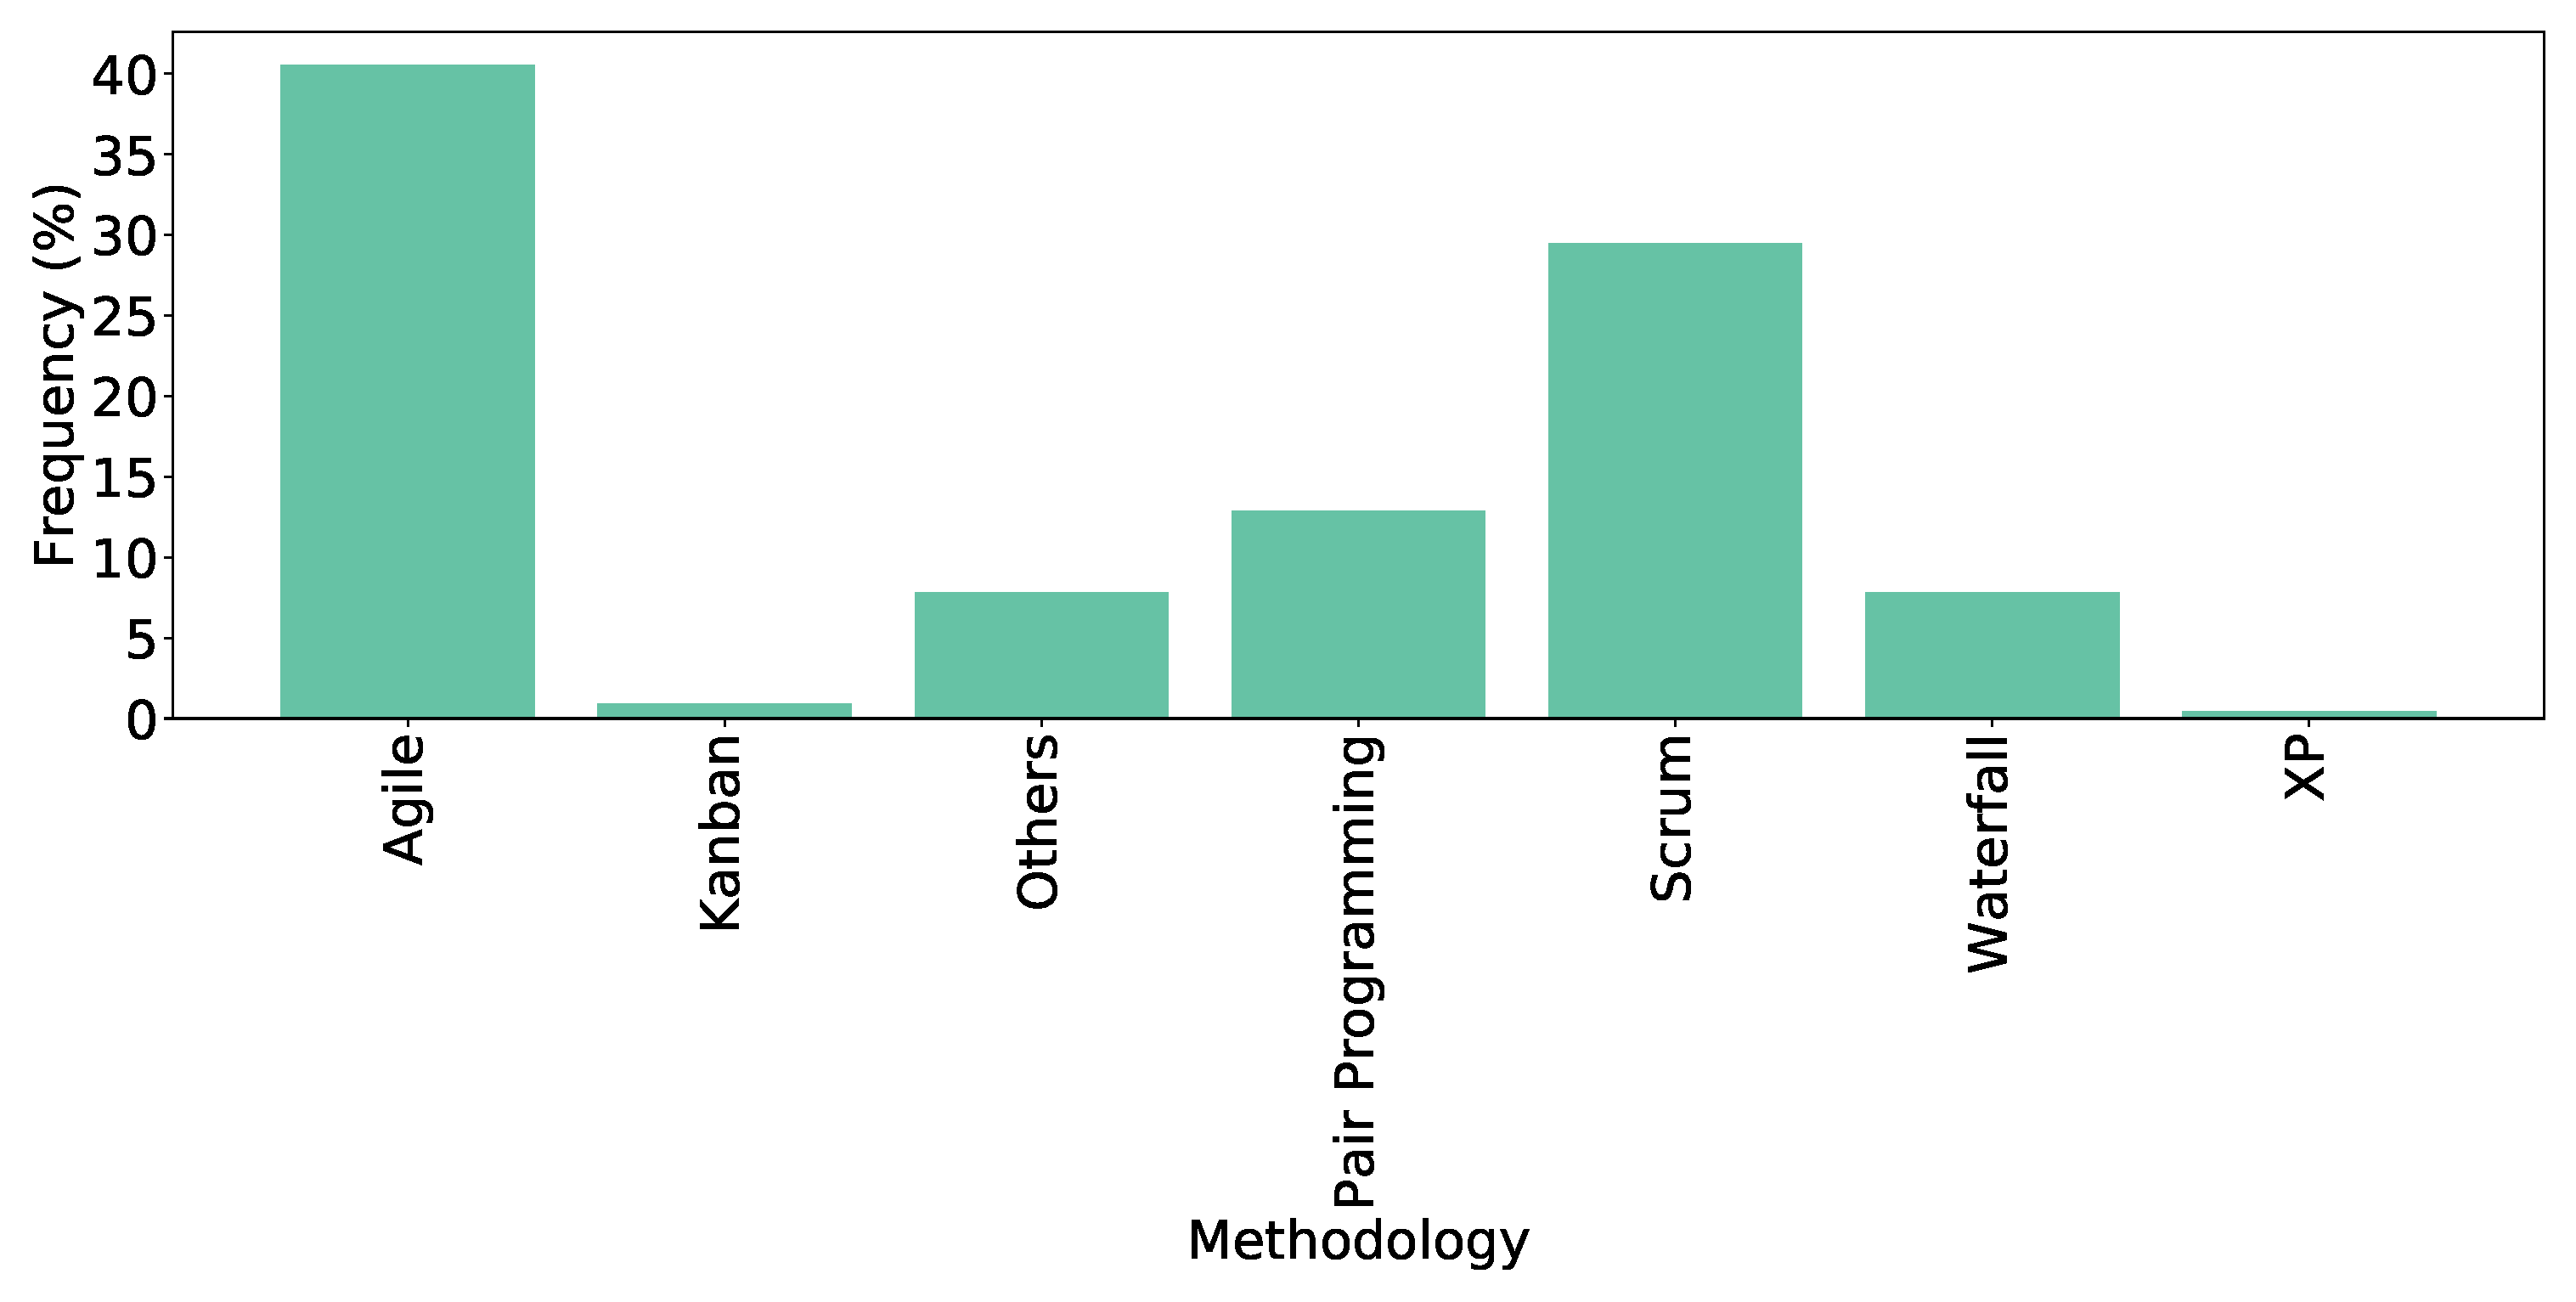
\includegraphics[scale=0.1]{Figures/Respondents_Methodology}
            \caption{Software development methodologies (Q6)}
            \label{fig:methodologies}
    \end{subfigure}
    \begin{subfigure}{0.45\textwidth}
          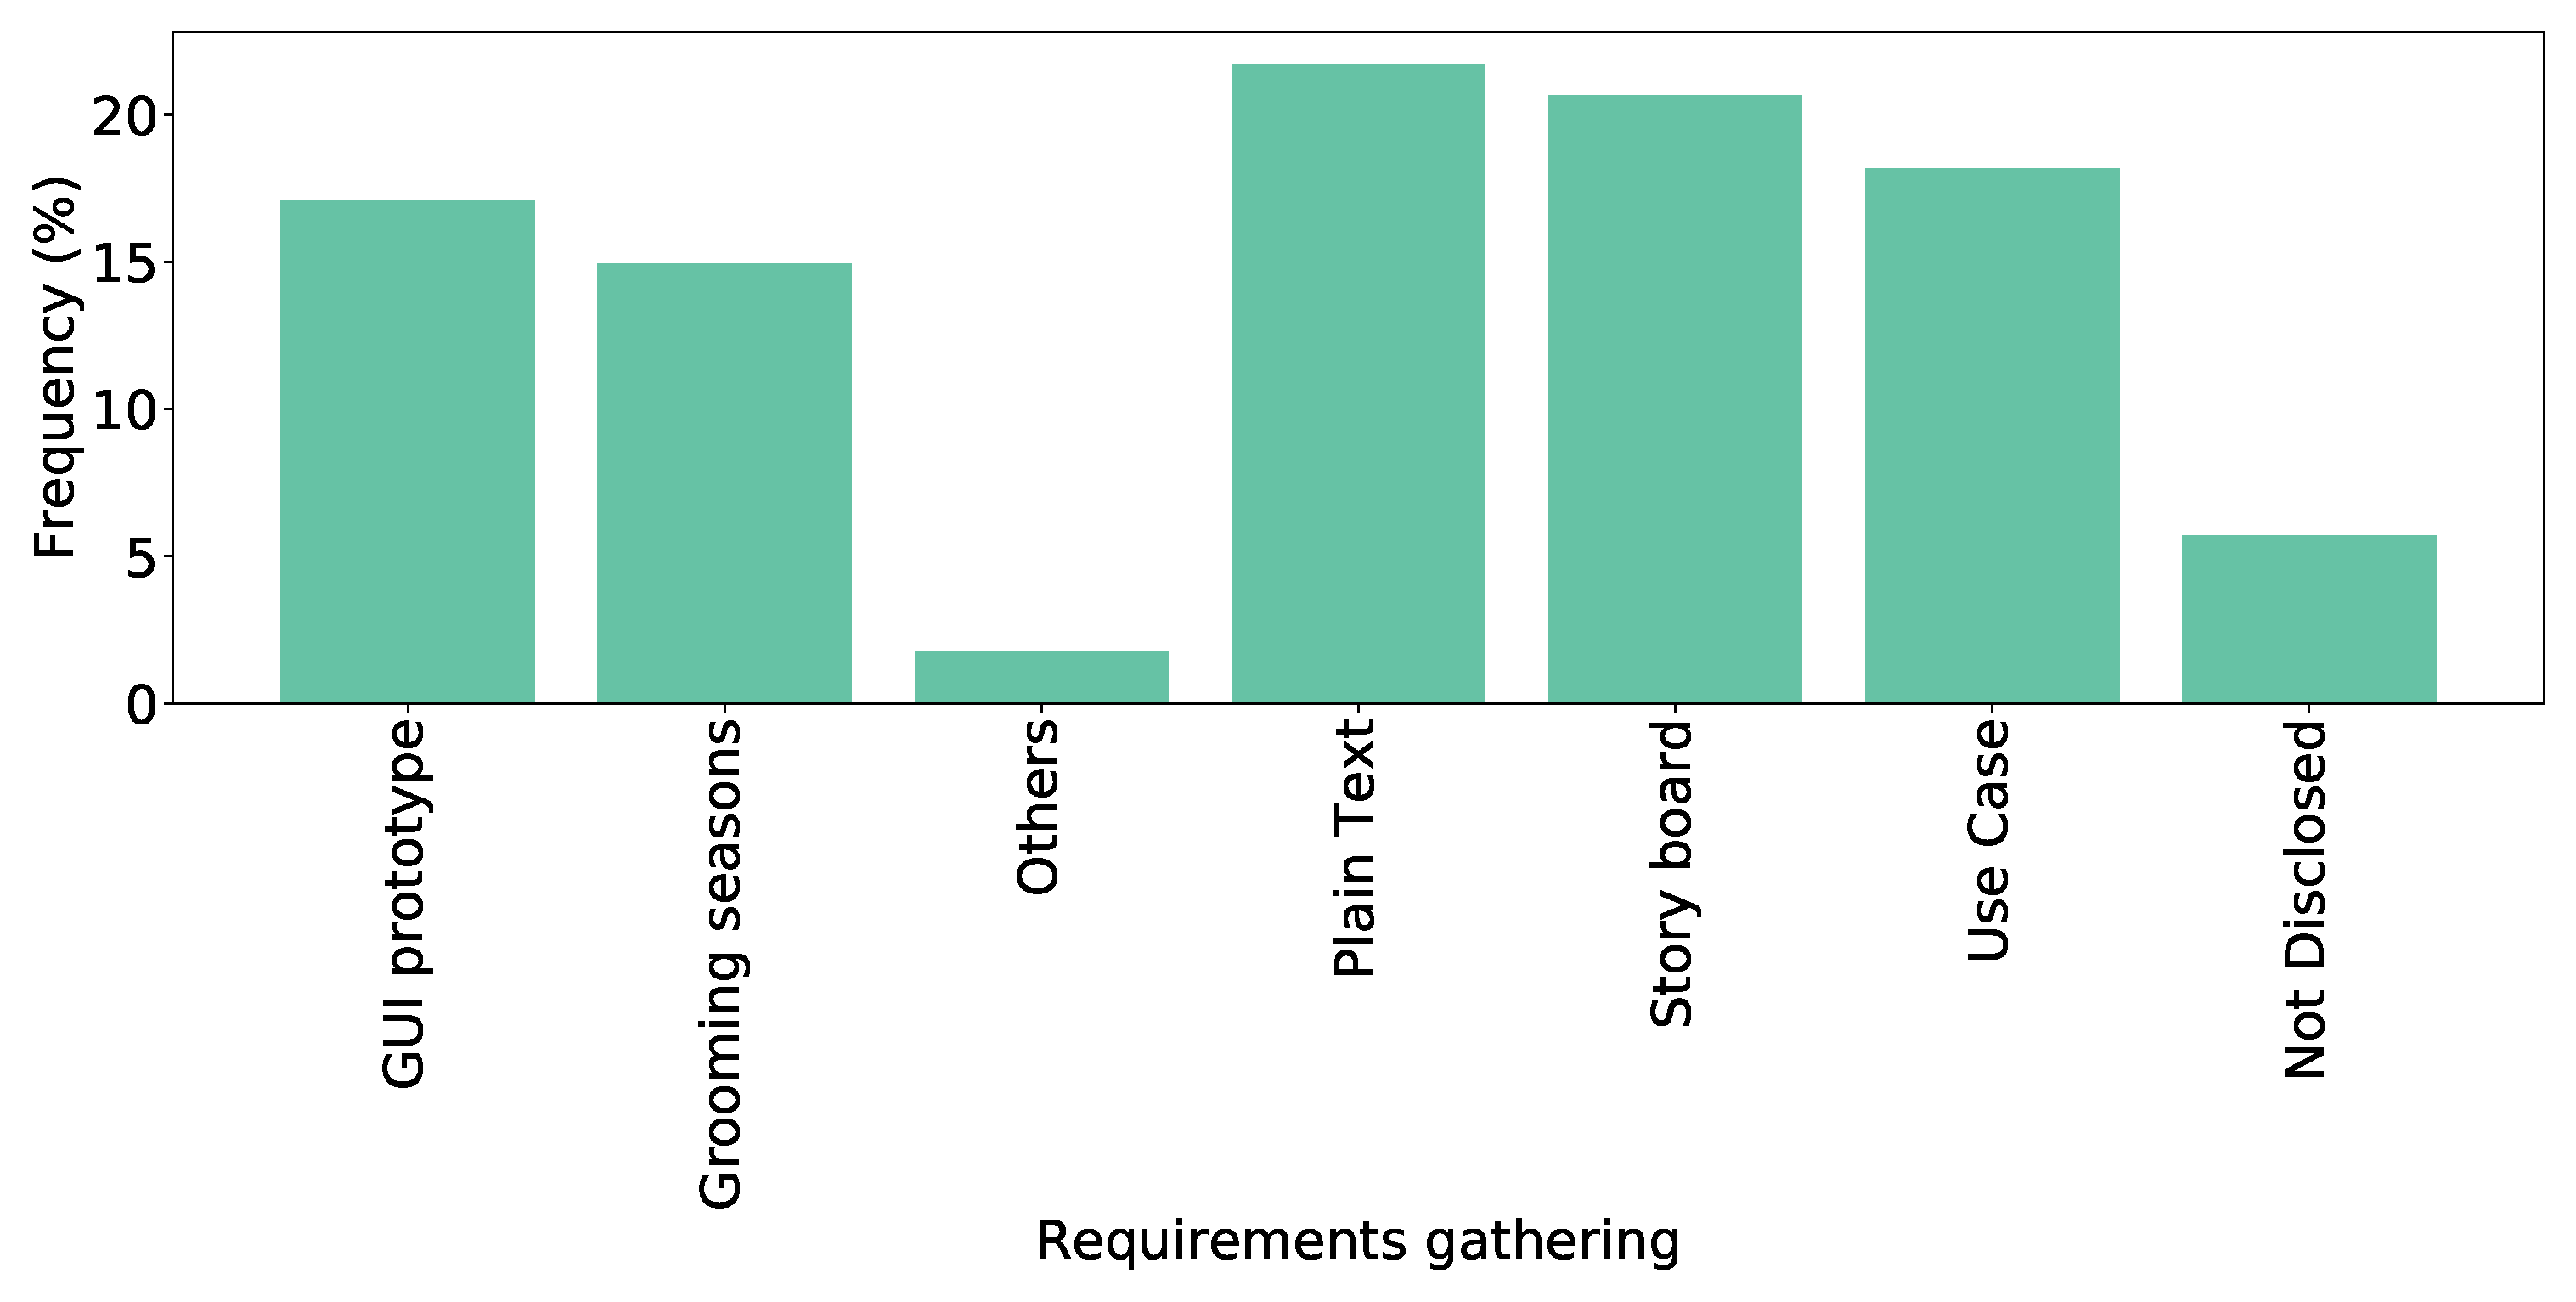
\includegraphics[scale=0.1]{Figures/Requirements_Gathering}
          \caption{Requirements gathering (Q7)}
          \label{fig:requirements}
    \end{subfigure}
    \begin{subfigure}{0.6\textwidth}
          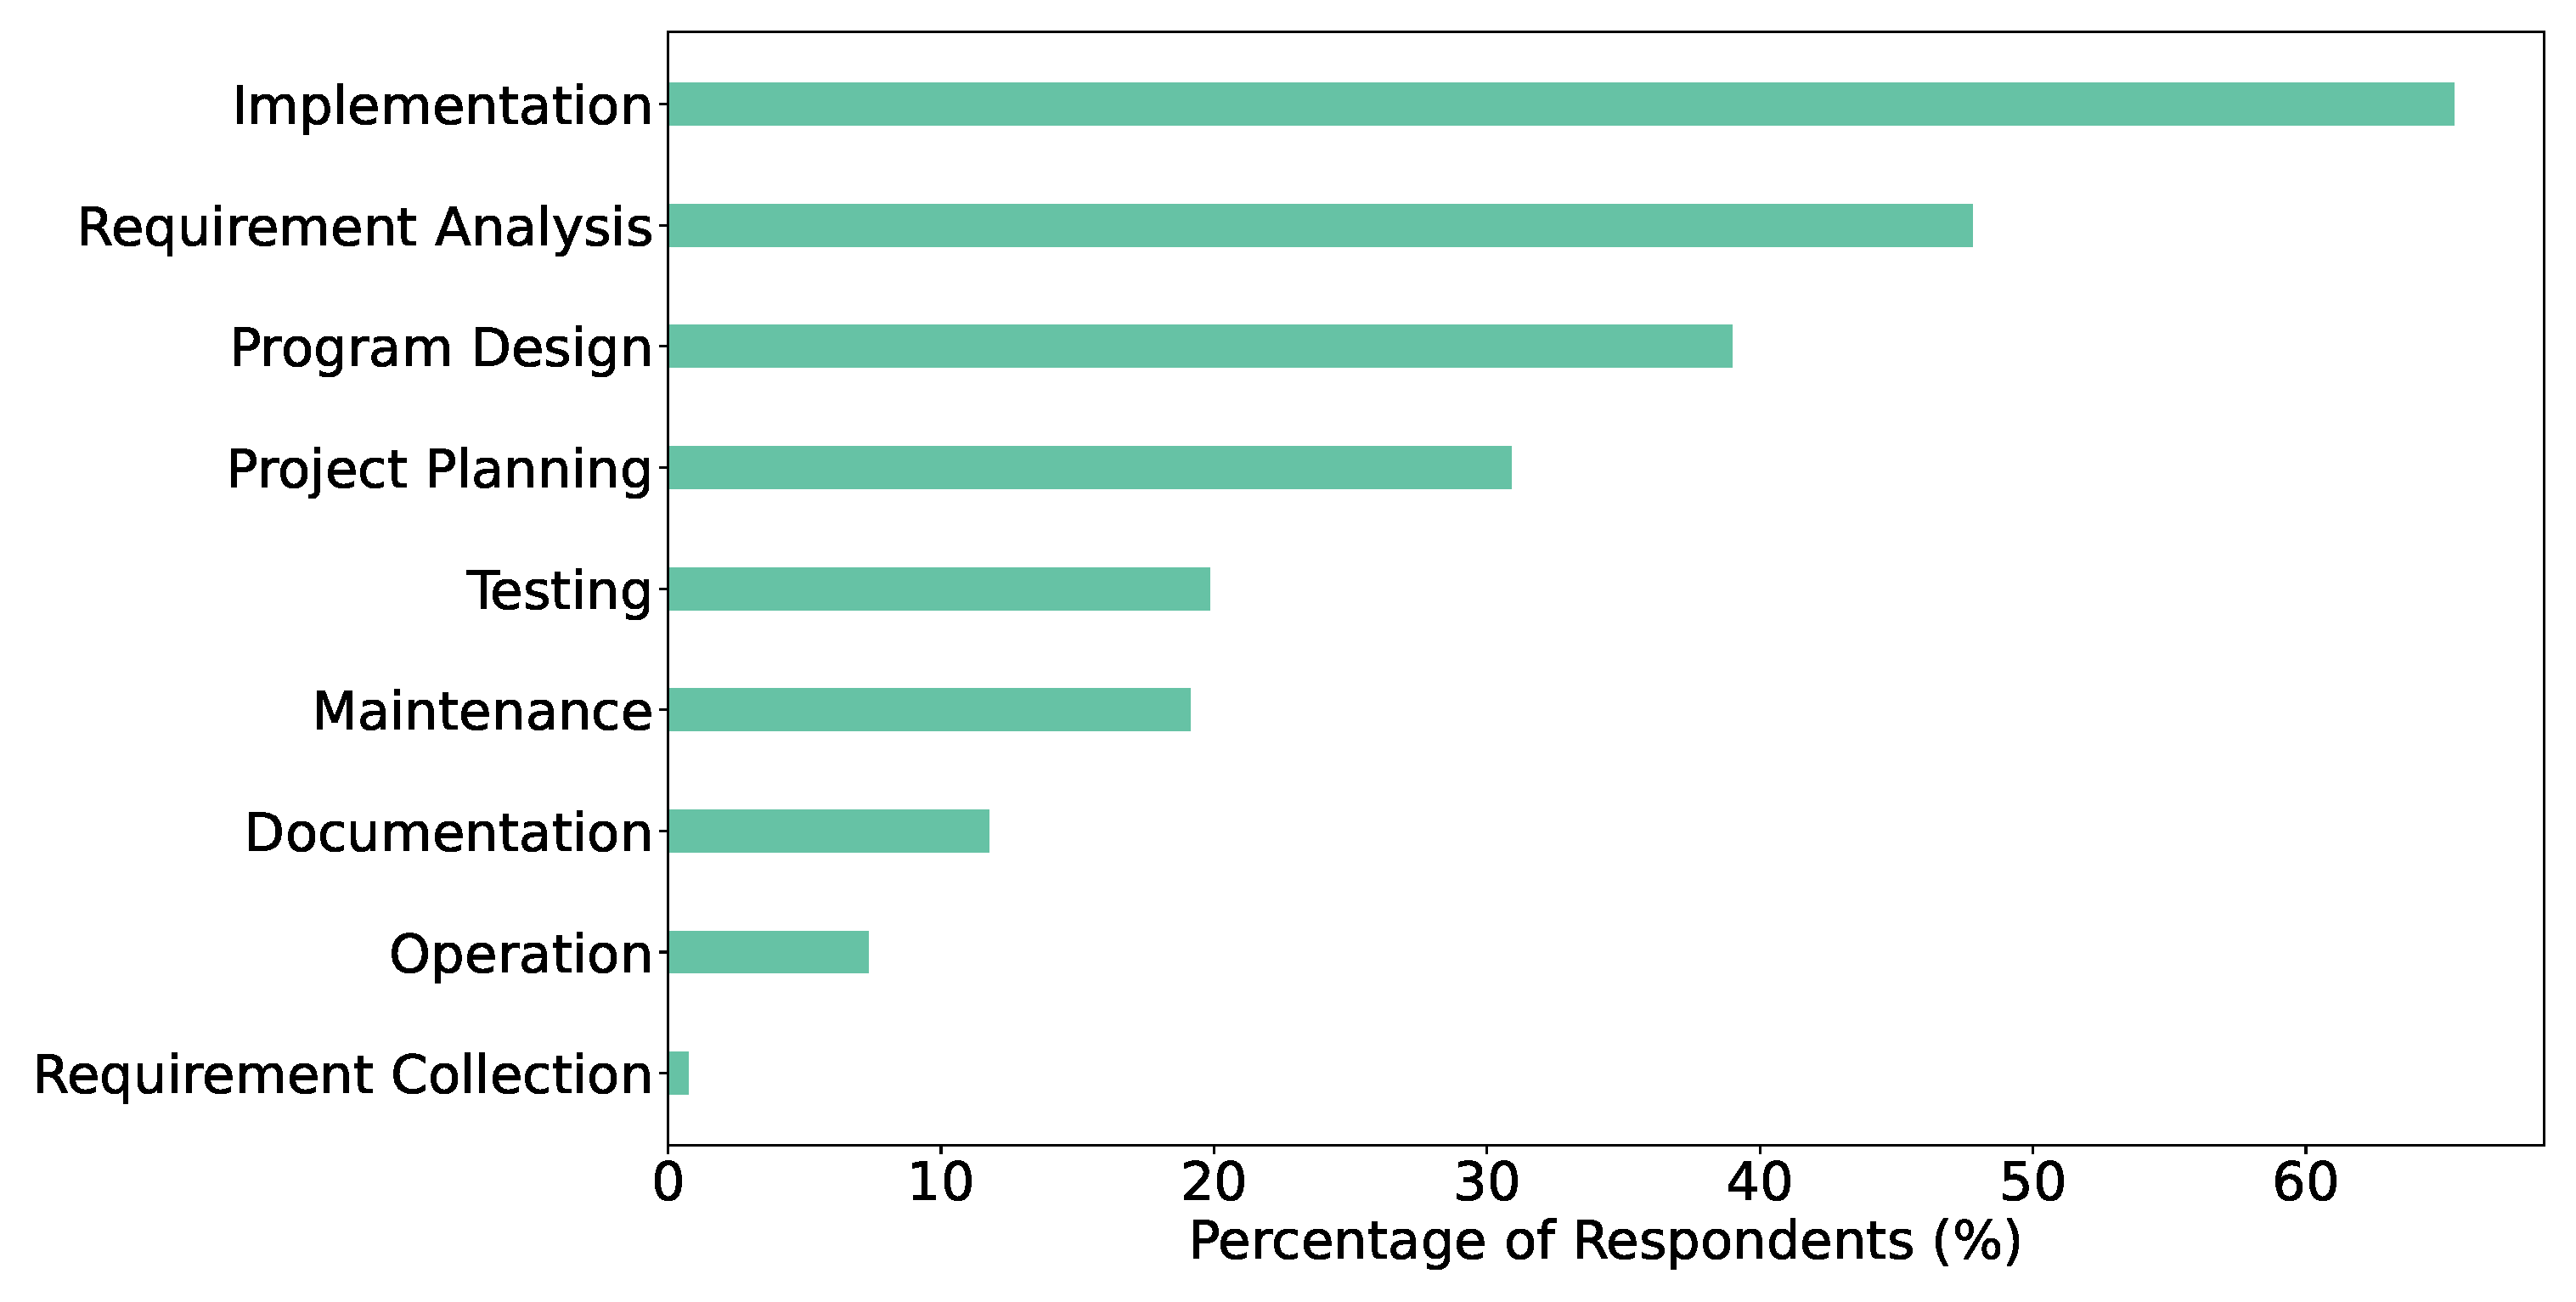
\includegraphics[scale=0.12]{Figures/Respondents_Activities}
          \caption{Timeline of Development Activities (Q8)}
          \label{fig:activities}
    \end{subfigure}
\end{figure}



% \begin{figure}[h]
% \centering
%   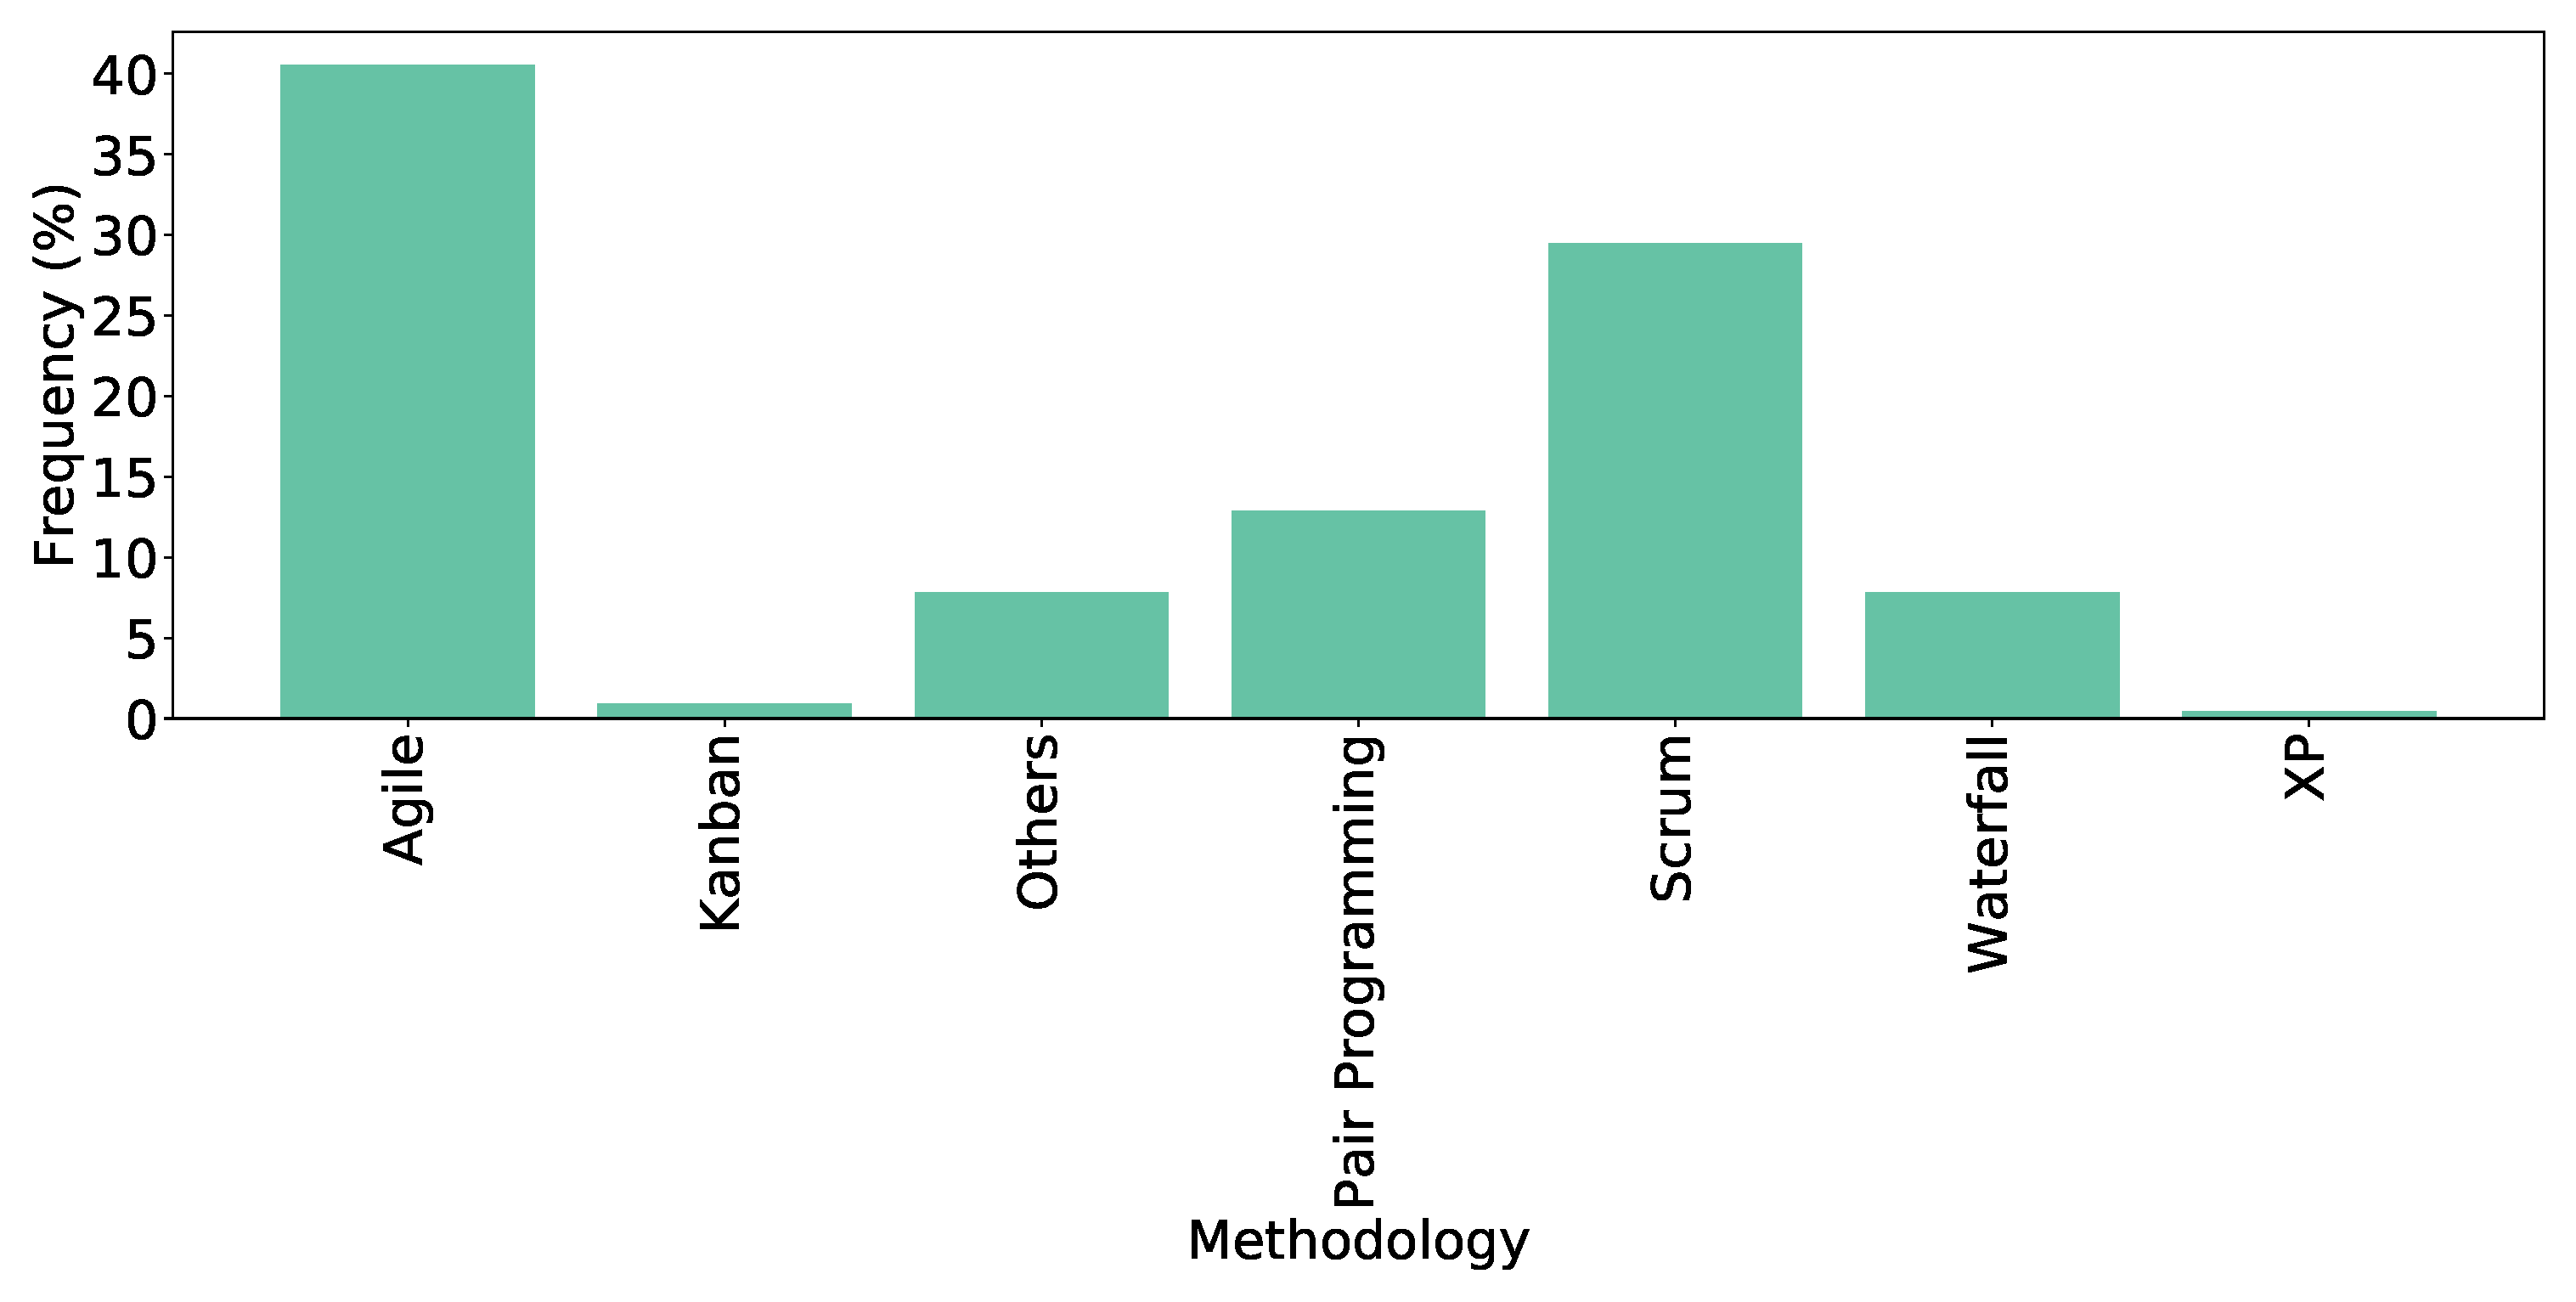
\includegraphics[scale=0.18]{Figures/Respondents_Methodology}
%   \caption{Software development methodologies (Q6)}
%   \label{fig:methodologies}
% \end{figure}

% 
% Through this question, we address the fundamental component of development
% practice in a company. We report the following relevant results:
% 
% \begin{itemize}
% \item Software development methodologies (Q 6).
% \item Requirements gathering (Q 7).
% \item Most time-consuming software development activities (Q 8).
% \end{itemize}
% 
% 
% \paragraph{Software development methodologies}
\nd\bf{$\bullet$ Requirements gathering (Q7).} The most critical activity that always arises
during software development is collecting and analyzing the requirements of a
system. Usually, the outcome of the analysis is presented before the client and
modified according to their feedback. The more clear and detailed requirements
are, the higher the possibility of building software that conducts the client’s
anticipation. Corresponding to Figure \ref{fig:requirements}, using plain text
(44\%) and storyboard (41\%) are the most widely used requirement gathering
techniques among our survey participants. The other relevant techniques include
use case (36\%), GUI prototype (35\%), grooming session (30\%), etc. 
% Here we see
% an appreciable percentage of software practitioners prefer plain text to collect
% requirements rather than using standard techniques. 
% This is an important finding
% that requires further analysis for causes and to analyze the potential effects
% of not practicing standard requirements gathering techniques frequently.

% \begin{figure}[h]
% \centering
%   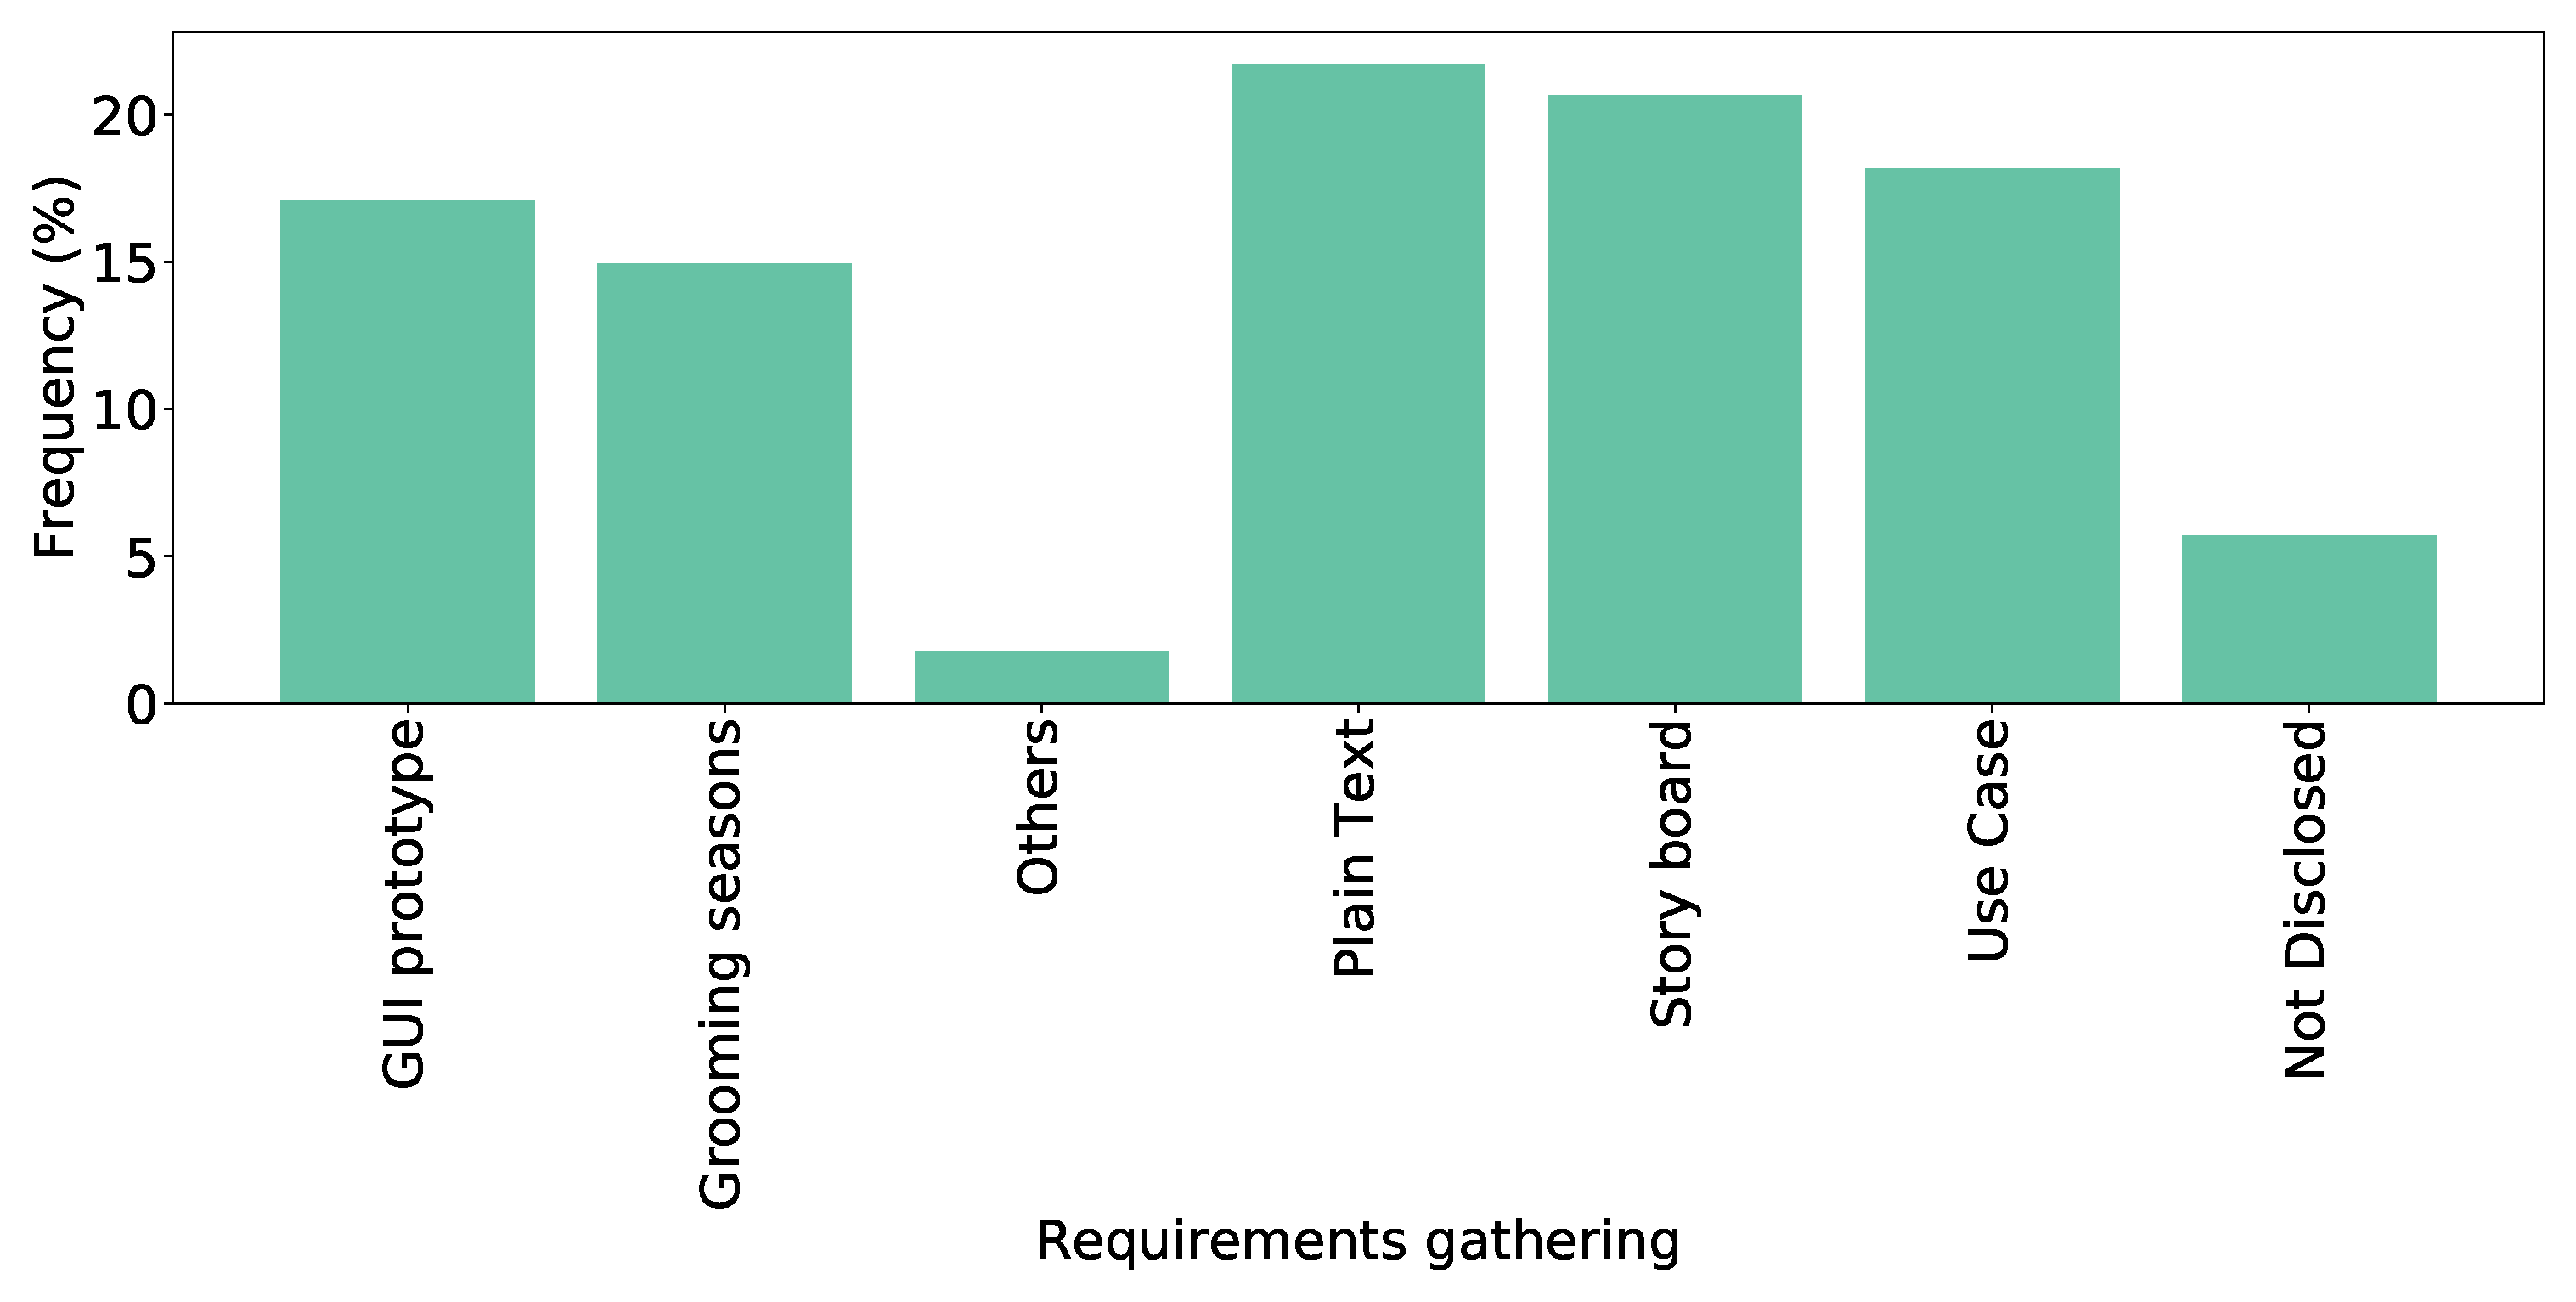
\includegraphics[scale=0.18]{Figures/Requirements_Gathering}
%   \caption{Requirements gathering (Q7)}
%   \label{fig:requirements}
% \end{figure}
% \begin{figure}[h]
% \centering
%   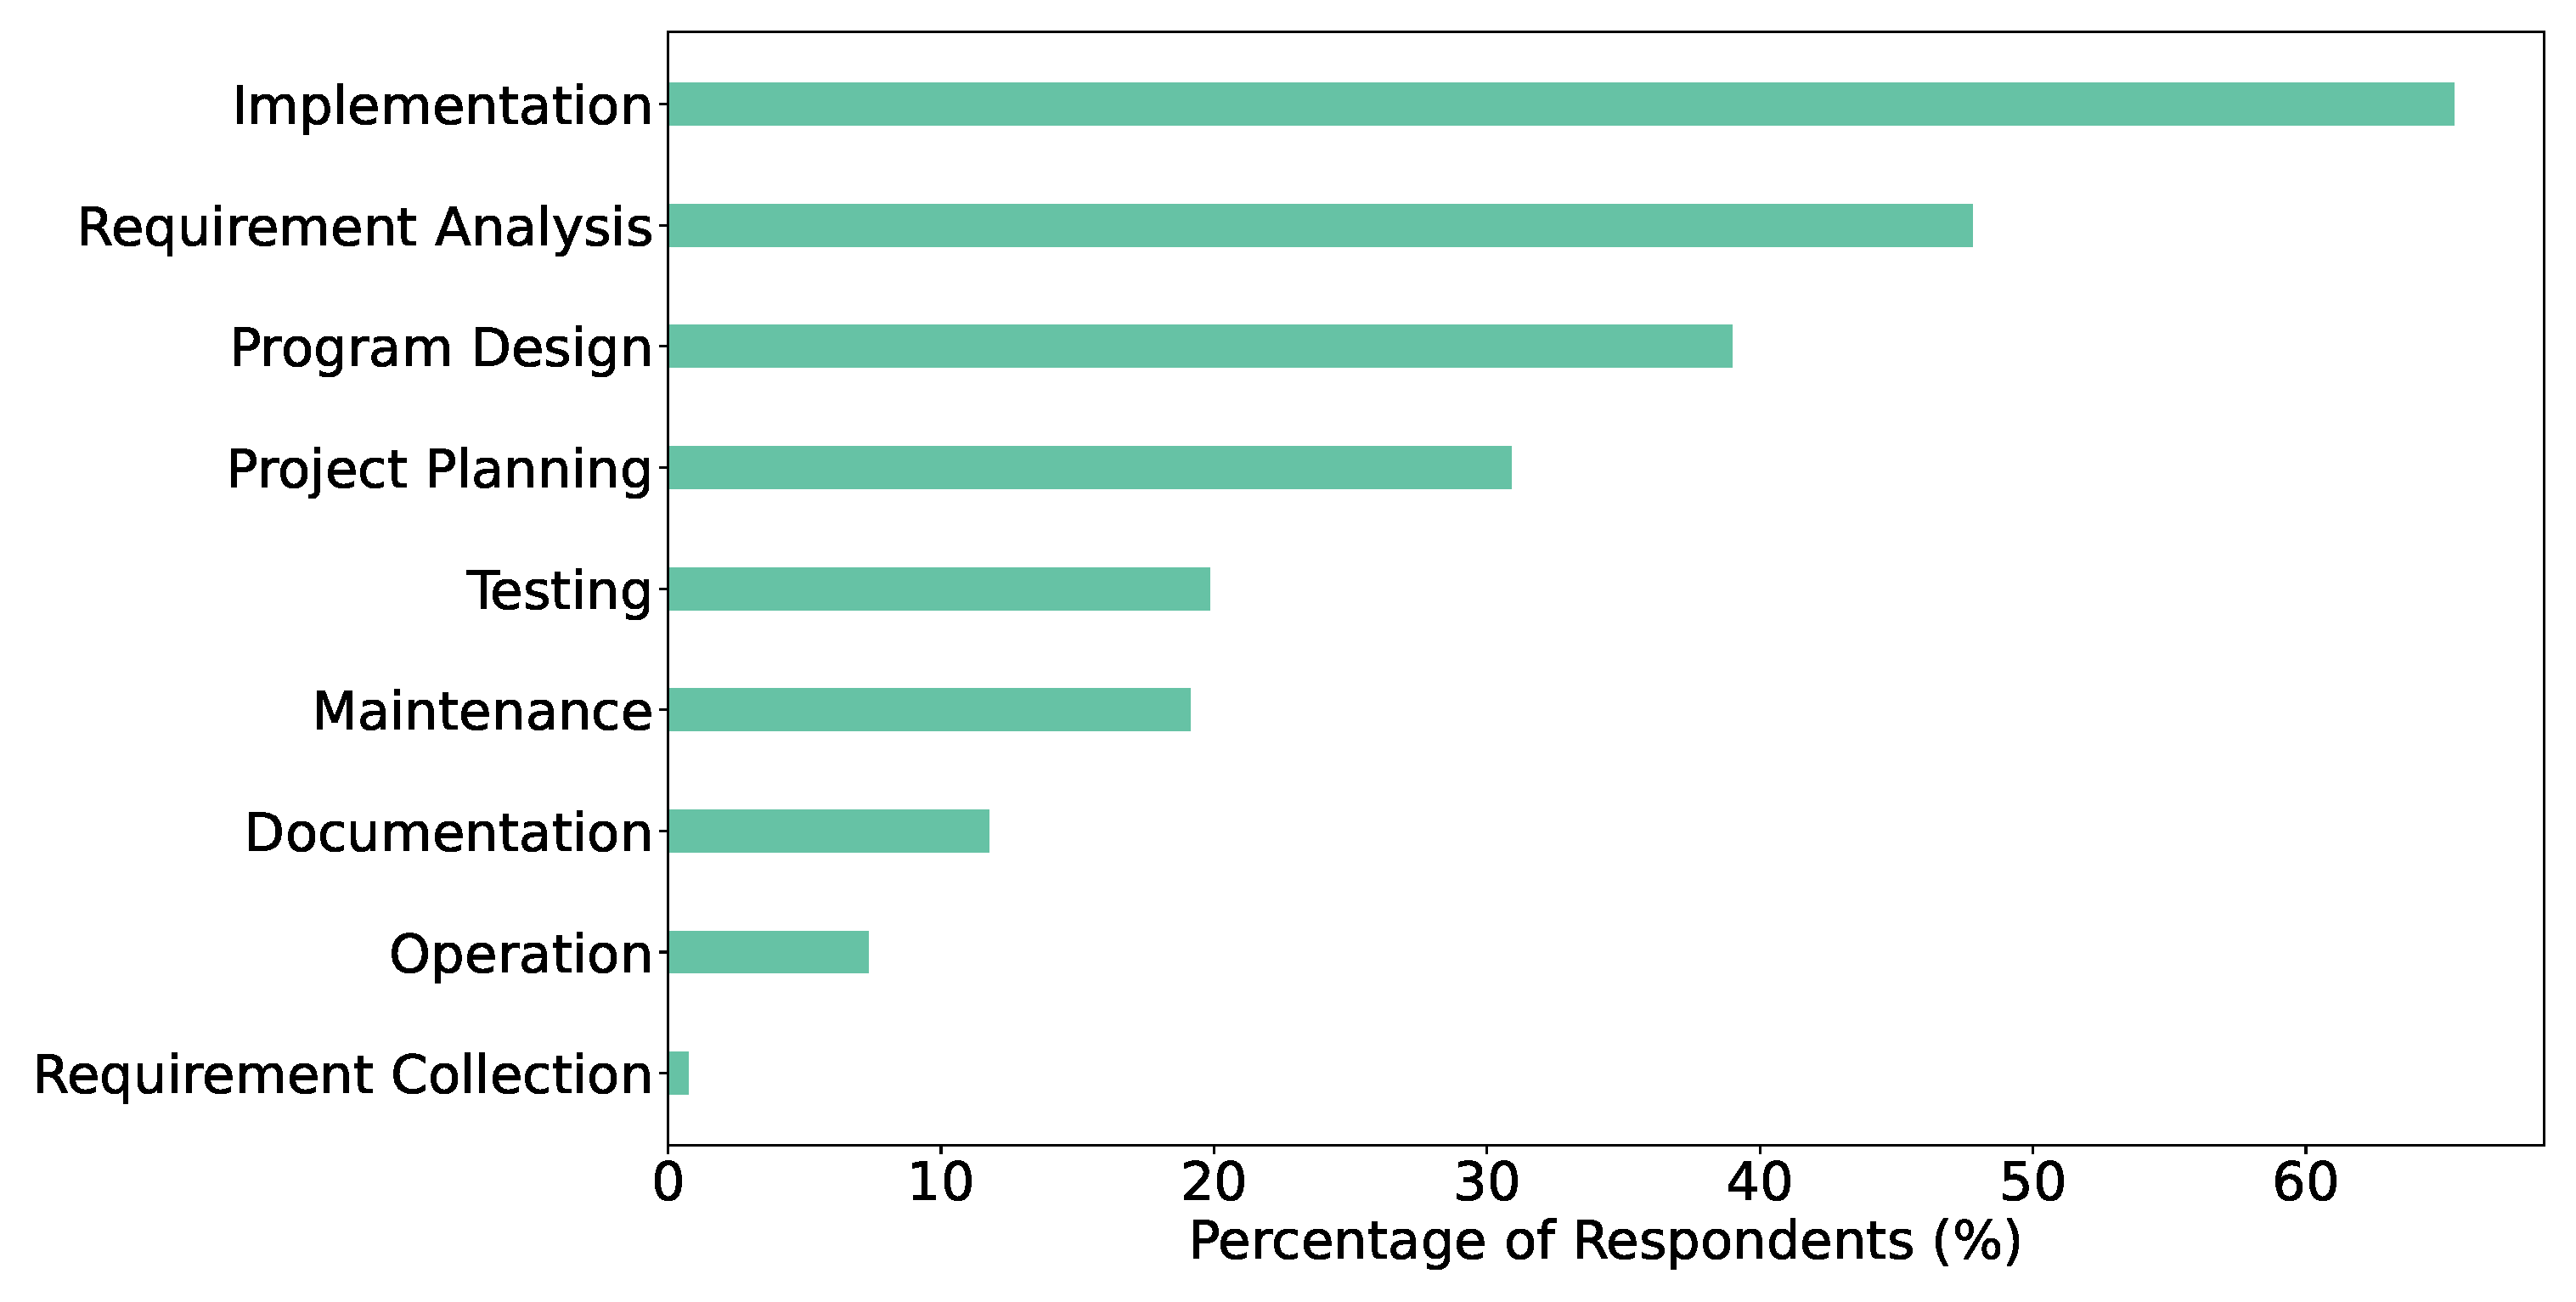
\includegraphics[scale=0.2]{Figures/Respondents_Activities}
%   \caption{Timeline of Development Activities (Q8)}
%   \label{fig:activities}
% \end{figure}

\nd\bf{$\bullet$ Timeline of Development Activities (Q8).} According to 65\% of our respondents, most of
the time is spent in the implementation stage, whereas the requirement analysis
stage requires the second most according to 45\% response. The other usages are
program design (37\%), project planning (30\%), testing (19\%), maintenance
(17\%), etc. There is no significant correlation between software development
methodologies (Q6) and the most time-consuming development activities (Q8) based on Cram\'{e}r's V \citep{Cramer1946} analysis. Cram\'{e}r's V 
calculates the association between two nominal
variables using Pearson's chi-squared statistic~\citep{Sheskin2007}.


% 
% It may happen that there could be a correlation between software development
% methodologies (Q6) and the most time-consuming development activities (Q8). 
% Thus we have
% calculated the Cram\'{e}r's V \citep{Cramer1946} between the choice of software
% development methodologies and most time spent activity of the respondents.
% Cram\'{e}r's V calculates the measure of association between two nominal
% variables~\citep{Sheskin2007}. However, we have not found any significant
% correlation.



% We guessed that there might be a relation between developers' experience and
% their activities. It is a general idea that senior developers spend most of
% their time in requirement specification and design activities, where junior
% developers spend their time implementing the solution. For analysis purposes, we
% divided our respondents into two groups based on their professional experience.
% The two groups are 1) Senior: Developers with more than 5 years of experience 2)
% Junior: Developers having less than 5 years of experience. We plotted the most
% time spent activity for the above-mentioned two groups in Figure
% \ref{fig:activity and seniority}. We can see that our anticipation is right.
% Junior developers are mostly engaged in the implementation, where senior
% developers are engaged with requirement specifications.
% \anindya{Do you consistently imply coding/development by implementation? In SE, it has a different meaning.}\partha{`Implementation' was one of the options of this closed question. It seems like respondents used it to mean coding/development. One of the responses to another question was `Implementation time carefulness and maintaining a well-developed coding standard.' Though I am not sure, it seems he means coding/development here}

% \begin{figure}[h]
% \centering
%   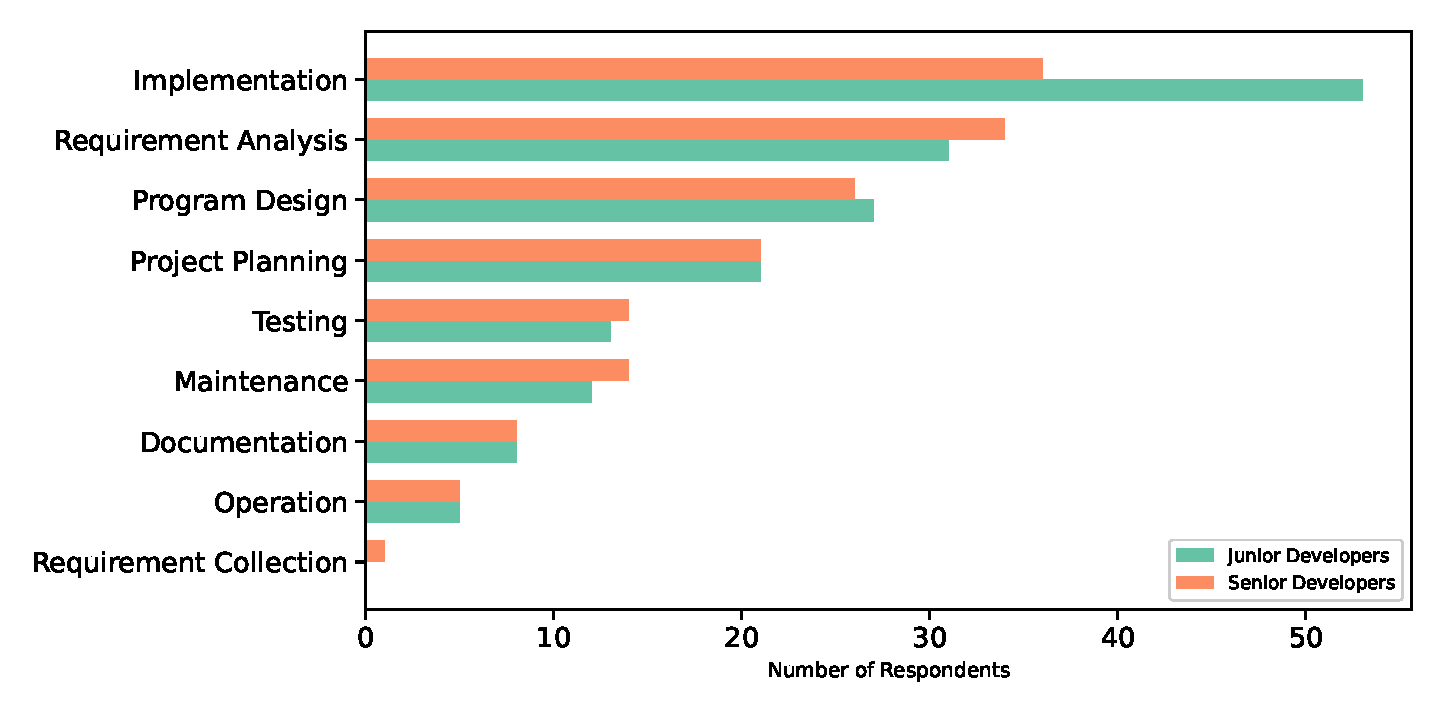
\includegraphics[scale=0.4]{Figures/Activity_and_Seniority.eps}
%   \caption{Relation between seniority and activity}
%   \label{fig:activity and seniority}
% \end{figure}

\begin{tcolorbox}[flushleft upper,boxrule=1pt,arc=0pt,left=0pt,right=0pt,top=0pt,bottom=0pt,colback=white,after=\ignorespacesafterend\par\noindent]
\nd\it{\bf{RQ1-D1. Software development methodologies used.}} To provide
software services, companies prefer the Agile approach most followed by Scrum
and also collect requirements via plain text in a high percentage. Besides,
developers of the Bangladeshi SE industry generally spend more time on
implementation-related activities than planning and testing. 
\end{tcolorbox}
%\boxtext{Developers of the Bangladeshi SE industry generally spend more time on implementation-related activities than planning and testing.}
